% system_cut.tex — ONE source, ONE rendered SVG (system_cut.svg), embedded in ../concurrent_system.md.
%
% A generic memory-mapped system: kernels A and B, an on-chip memory, a crossbar, a host.  Three
% nested scopes -- the System (the whole pysim graph), the DUT (the default cut: what is
% synthesized), and each device (one sub-top, one IP) -- and each block coloured by how the flow
% realizes it: Vitis HLS, hand-written RTL, vendor IP, or a testbench C++ model.
%
% Render: bash render.sh   (MiKTeX pdflatex -> PDF -> dvisvgm --pdf -> SVG)
\documentclass[tikz,border=6pt]{standalone}
\usepackage{tikz}
\usetikzlibrary{arrows.meta,positioning,calc,fit,backgrounds}

% Theme-neutral palette (pale fills, explicit strokes): the SVG is viewed on light and dark pages.
\definecolor{hlsfill}{HTML}{DCE9F7}  \definecolor{hlsline}{HTML}{2C6FB5}   % Vitis HLS -> csynth
\definecolor{rtlfill}{HTML}{DFF0D8}  \definecolor{rtlline}{HTML}{3C7A2E}   % hand-written RTL leaf
\definecolor{ipfill}{HTML}{EADCF2}   \definecolor{ipline}{HTML}{7A4A9A}    % vendor IP (create_ip)
\definecolor{tbfill}{HTML}{F2E6D0}   \definecolor{tbline}{HTML}{9A6B1F}    % testbench C++ model
\definecolor{dutline}{HTML}{1F3B5C}
\definecolor{devline}{HTML}{555555}
\definecolor{sysline}{HTML}{8A8A8A}
\definecolor{inkgray}{HTML}{444444}

\begin{document}
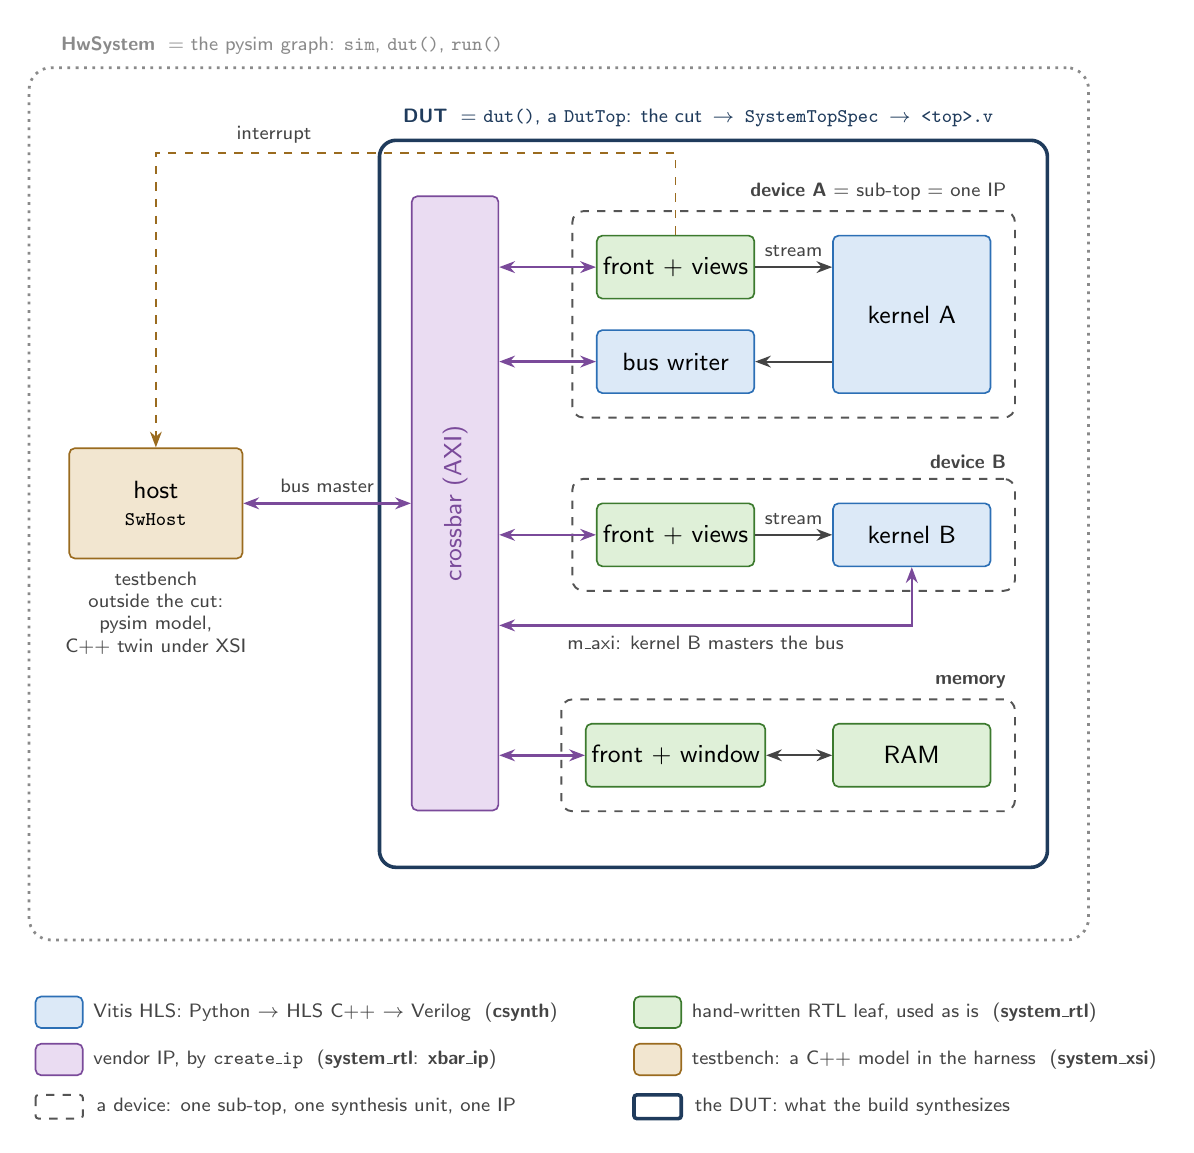
\begin{tikzpicture}[
  font=\sffamily\small,
  blk/.style   = {draw, rounded corners=2pt, minimum height=8mm, align=center, line width=0.6pt,
                  inner sep=2pt},
  hls/.style   = {blk, fill=hlsfill, draw=hlsline, minimum width=20mm},
  rtl/.style   = {blk, fill=rtlfill, draw=rtlline, minimum width=20mm},
  ip/.style    = {blk, fill=ipfill, draw=ipline},
  tb/.style    = {blk, fill=tbfill, draw=tbline, minimum width=22mm},
  data/.style  = {-{Stealth[length=2mm]}, line width=0.7pt, draw=inkgray},
  bus/.style   = {{Stealth[length=2mm]}-{Stealth[length=2mm]}, line width=0.9pt, draw=ipline},
  irq/.style   = {-{Stealth[length=2mm]}, line width=0.6pt, draw=tbline, dashed},
  device/.style= {draw=devline, dashed, rounded corners=4pt, line width=0.7pt},
  dut/.style   = {draw=dutline, rounded corners=6pt, line width=1.3pt},
  sys/.style   = {draw=sysline, dotted, rounded corners=8pt, line width=1.0pt},
  lbl/.style   = {font=\sffamily\scriptsize, text=inkgray},
  tag/.style   = {font=\sffamily\scriptsize\bfseries},
]

% ---------------- the crossbar (vendor IP) ---------------------------------------------------
\node[ip, minimum width=11mm, minimum height=78mm] (xbar) at (3.2, 0.3) {};
\node[font=\sffamily\small, rotate=90, text=ipline] at (xbar) {crossbar (AXI)};

% ---------------- device A: front + views, kernel A, the bus writer acting for it -----------
\node[rtl]  (fa) at (6.0,  3.3) {front + views};
\node[hls]  (wa) at (6.0,  2.1) {bus writer};
\node[hls, minimum height=20mm]  (ka) at (9.0,  2.7) {kernel A};
\draw[data] (fa.east) -- node[lbl, above, sloped] {stream} (ka.west |- fa.east);
\draw[data] (ka.west |- wa.east) -- (wa.east);
\draw[bus]  (xbar.east |- fa.west) -- (fa.west);
\draw[bus]  (wa.west) -- (xbar.east |- wa.west);
\begin{scope}[on background layer]
  \node[device, fit=(fa)(wa)(ka), inner sep=3mm] (devA) {};
\end{scope}
\node[lbl, anchor=south east] at (devA.north east) {\textbf{device A} = sub-top = one IP};

% ---------------- device B: front + views, kernel B (which also masters the bus) -------------
\node[rtl]  (fb) at (6.0, -0.1) {front + views};
\node[hls]  (kb) at (9.0, -0.1) {kernel B};
\draw[data] (fb.east) -- node[lbl, above] {stream} (kb.west);
\draw[bus]  (xbar.east |- fb.west) -- (fb.west);
\draw[bus]  (kb.south) |- node[lbl, pos=0.75, below] {m\_axi: kernel B masters the bus} (xbar.east |- 0,-1.25);
\begin{scope}[on background layer]
  \node[device, fit=(fb)(kb), inner sep=3mm] (devB) {};
\end{scope}
\node[lbl, anchor=south east] at (devB.north east) {\textbf{device B}};

% ---------------- the memory: front + window, RAM ---------------------------------------------
\node[rtl]  (fm) at (6.0, -2.9) {front + window};
\node[rtl]  (rm) at (9.0, -2.9) {RAM};
\draw[data, {Stealth[length=2mm]}-{Stealth[length=2mm]}] (fm.east) -- (rm.west);
\draw[bus]  (xbar.east |- fm.west) -- (fm.west);
\begin{scope}[on background layer]
  \node[device, fit=(fm)(rm), inner sep=3mm] (devM) {};
\end{scope}
\node[lbl, anchor=south east] at (devM.north east) {\textbf{memory}};

% ---------------- the DUT: the default cut -> SystemTopSpec -> <top>.v ----------------------
\begin{scope}[on background layer]
  \node[dut, fit=(xbar)(devA)(devB)(devM), inner xsep=4mm, inner ysep=7mm] (dut) {};
\end{scope}
\node[tag, text=dutline, anchor=south west] at ($(dut.north west)+(2mm,0.3mm)$)
     {DUT \;\textmd{= \texttt{dut()}, a \texttt{DutTop}: the cut \,$\to$\, \texttt{SystemTopSpec} \,$\to$\, \texttt{<top>.v}}};

% ---------------- the host: the testbench -----------------------------------------------------
\node[tb, minimum height=14mm] (host) at (-0.6, 0.3) {host\\[-1pt]\scriptsize\texttt{SwHost}};
\draw[bus] (host.east) -- node[lbl, above] {bus master} (xbar.west |- host.east);
\draw[irq] (fa.north) |- (host.north |- 0,4.75) -- (host.north);
\node[lbl, anchor=south] at (0.9,4.75) {interrupt};
\node[lbl, align=center, anchor=north] at (host.south)
     {\\[-2pt]testbench\\outside the cut:\\pysim model,\\C++ twin under XSI};

% ---------------- the System: the whole pysim graph -----------------------------------------
\begin{scope}[on background layer]
  \node[sys, fit=(host)(dut), inner xsep=5mm, inner ysep=9mm] (sys) {};
\end{scope}
\node[tag, text=sysline, anchor=south west] at ($(sys.north west)+(3mm,0.3mm)$)
     {HwSystem \;\textmd{= the pysim graph: \texttt{sim}, \texttt{dut()}, \texttt{run()}}};

% ---------------- legend ---------------------------------------------------------------------
\begin{scope}[shift={($(sys.south west)+(0.4,-0.9)$)}, every node/.style={font=\sffamily\scriptsize}]
  \node[hls, minimum width=6mm, minimum height=4mm] (l1) at (0,0) {};
  \node[anchor=west, text=inkgray] at (l1.east) {Vitis HLS: Python $\to$ HLS C++ $\to$ Verilog \ (\textbf{csynth})};
  \node[rtl, minimum width=6mm, minimum height=4mm] (l2) at (7.6,0) {};
  \node[anchor=west, text=inkgray] at (l2.east) {hand-written RTL leaf, used as is \ (\textbf{system\_rtl})};
  \node[ip, minimum width=6mm, minimum height=4mm] (l3) at (0,-0.6) {};
  \node[anchor=west, text=inkgray] at (l3.east) {vendor IP, by \texttt{create\_ip} \ (\textbf{system\_rtl}: \textbf{xbar\_ip})};
  \node[tb, minimum width=6mm, minimum height=4mm] (l4) at (7.6,-0.6) {};
  \node[anchor=west, text=inkgray] at (l4.east) {testbench: a C++ model in the harness \ (\textbf{system\_xsi})};
  \draw[device, rounded corners=1pt] (-0.3,-1.05) rectangle (0.3,-1.35);
  \node[anchor=west, text=inkgray] at (0.35,-1.2) {a device: one sub-top, one synthesis unit, one IP};
  \draw[dut, rounded corners=1pt] (7.3,-1.05) rectangle (7.9,-1.35);
  \node[anchor=west, text=inkgray] at (7.95,-1.2) {the DUT: what the build synthesizes};
\end{scope}

\end{tikzpicture}
\end{document}
